%CS-113 S18 HW-6 Solutions
%Released: 17-April-2018
%Authors: Abdullah Zafar

\documentclass[addpoints]{exam}

% Header and footer.
\pagestyle{headandfoot}
\runningheadrule
\runningfootrule
\runningheader{CS 113 Discrete Mathematics}{Homework VI}{Spring 2018}
\runningfooter{}{Page \thepage\ of \numpages}{}
\firstpageheader{}{}{}

\boxedpoints
\printanswers
\usepackage[table]{xcolor}
\usepackage{amsfonts,graphicx,amsmath,hyperref,amssymb}
\usepackage{tikz}
\hypersetup{
    colorlinks=true,
    linkcolor=blue,
    urlcolor=cyan,
}

\title{Habib University\\CS-113 Discrete Mathematics\\Spring 2018\\HW 6 Solutions}

\date{Released: 17th April, 2018}


\begin{document}
\maketitle

\begin{questions}



\question
Prove that a graph of $n$ vertices and $n-1$ edges has a vertex of degree 1 or an isolated vertex.
  \begin{solution}
  Suppose, for the sake of absurdity, that all vertices of the graph are of degree at least $2$. We know, by the \textbf{Handshake Theorem}, that the total number of edges in this graph should be half the number of total degrees, i.e., at least $\frac{2n}{2}=n$. But the graph has $n-1$ edges only. Therefore, our initial assumption must be wrong. 
  \end{solution}

\question 
Prove that a graph $G$ is $2$-connected \textbf{iff} for every triple $(x,y,z)$ of distinct vertices, $G$ has an $(x,z)$ path through $y$.

(A graph is $2$-connected if removing at least 2 vertices (and associated edges) disconnects it or produces a graph with a single vertex)  


  \begin{solution}
  
  To prove: \textit{If for every triple (x,y,z) of distinct vertices, G has an (x,z) path through y, then G is 2-connected.}
  
  Suppose, for sake of absurdity, that $G$ is 1-connected. Remove any cut vertex $a$ from $G$ to get $G' = G - \{a\}$. Since $G'$ has at least one more component than $G$, it must have at least one pair of non-connected vertices $b$ and $c$ (there is no path from $b$ to $c$) which were connected in $G$ via $a$. By our initial assumption, there exists a path from $a$ to $c$ via $b$. Since this path cannot go through $a$ (simple path), $b$ and $c$ must be connected through another vertex. Therefore, our assumption that $G$ is 1-connected must be wrong.
  
  
  To prove: \textit{If G is 2-connected, then for every triple(x,y,z) of distinct vertices, G has an (x,z) path through y.}
  
  We prove the contrapositive: \textit{If for some triple (x,y,z), G does not have a (x,z) path through y, then G is at most 1-connected.}
  
  Consider the triple $(x,y,z)$ for which there is no $(x,z)$ path through $y$. Removing $x$ from the graph guarantess that there is no path from $y$ to $z$. Therefore, the graph must be at most 1-connected.
  
  \end{solution}
  
\question 
Are the following graphs isomorphic? Provide a mapping if they are, or explain why they are not.
\[
\begin{bmatrix}
0 & 1 & 1 & 0 & 0 & 0\\
1 & 0 & 1 & 1 & 0 & 0\\
1 & 1 & 0 & 0 & 0 & 0\\
0 & 1 & 0 & 0 & 1 & 1\\
0 & 0 & 0 & 1 & 0 & 1\\
0 & 0 & 0 & 1 & 1 & 0\\
\end{bmatrix}
\qquad
\begin{bmatrix}
0 & 0 & 1 & 0 & 1 & 0\\
0 & 0 & 0 & 1 & 0 & 1\\
1 & 0 & 0 & 0 & 1 & 0\\
0 & 1 & 0 & 0 & 0 & 1\\
1 & 0 & 1 & 0 & 0 & 1\\
0 & 1 & 0 & 1 & 1 & 0\\
\end{bmatrix}
\]

  \begin{solution}
  Let $a_i,i \in [1,6]$ be the row-wise vertices of the graph on the left, and $b_i,i \in [1,6]$ be the row-wise vertices of the graph on the right. Here is a mapping between the two sets of vertices:
  
   $a_1 \rightarrow b_1,a_2 \rightarrow b_5,a_3 \rightarrow b_3,a_4\rightarrow b_6,a_5 \rightarrow b_4,a_6 \rightarrow b_2$ 
   
   [There are 7 other correct mappings]
   
   
    
  \end{solution}

\question
The complement of a graph $G = (V,E)$ is the graph 

\[(V,\{\{x,y\} \subset V, x \not = y\} \;\backslash \;E)\]

A graph is \textit{self-complementary} if it is isomorphic to its complement.

\begin{parts}
	\part Prove that no simple graph with two or three vertices is self-complementary, without enumerating all isomorphisms of such simple graphs.
	G
	\begin{solution}
	Consider a graph $G$ and its complement $G'$. If $G$ is isomorphic to $G'$ then they must have the same number of edges. Therefore, the identity $\binom{n}{2} - e = e \rightarrow \binom{n}{2} = 2e$ where $n$ is the number of vertices and $e$ the number of edges of $G$, must hold. But neither $\binom{2}{2}$ nor $\binom{3}{2}$ is even. Therefore, the identity can not hold for $n=2,3$.  
	\end{solution}
	
	\part Give one example each of self-complementary simple graphs with 4 and 5 vertices.
	\end{parts}

   \begin{solution}
     
     \centering
     \begin{tabular}{c c}
    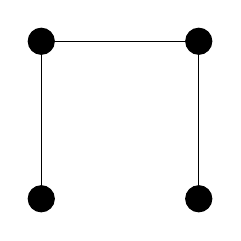
\begin{tikzpicture}[auto, node distance=2cm, every loop/.style={},
    thin,main node/.style={circle,draw,fill=black}]
    
    \node[main node] (1) {};
    \node[main node] (2) [left of=1] {};
    \node[main node] (3) [below of=2] {};
    \node[main node] (4) [right of=3] {};
    
    \path[every node/.style={font=\sffamily\small}]
    (1) edge node [left] {} (4)
    (2) edge node [right] {} (1)
    (3) edge node [right] {} (2);
    \end{tikzpicture}
    &\qquad \qquad
    	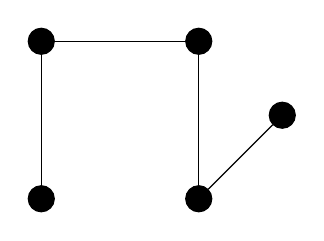
\begin{tikzpicture}[auto, node distance=2cm, every loop/.style={},
    	thin,main node/.style={circle,draw,fill=black}]
    	
    	\node[main node] (1) {};
    	\node[main node] (2) [left of=1] {};
    	\node[main node] (3) [below of=2] {};
    	\node[main node] (4) [right of=3] {};
    	\node[main node, node distance=1.5cm] (5) [above right of=4] {};
    	
    	\path[every node/.style={font=\sffamily\small}]
    	(1) edge node [right] {} (4)
    	(2) edge node [right] {} (1)
    	(3) edge node [right] {} (2)
    	(5) edge node [left] {} (4);
    	\end{tikzpicture}\\
     $n=4$ & \quad $n=5$ 
    \end{tabular}
  \end{solution}

\question 
Consider a graph $G$ with two sets of vertices $M$ and $N$ and a set of undirected edges $E$ such that $\forall m\in M, n \in N(\{m,n\} \in E)$. Determine (and prove) all $|M|,|N|\in \mathbb{N}$ for which $G$ is
\begin{parts}
	\part Eulerian
	\begin{solution}
	An Euler cycle exists iff $|M|,|N| \geq 2$ are both even. This is because an Euler cycle exists iff all vertices are of even degree.  
	\end{solution}
	\part Hamiltonian
	\begin{solution}
	A Hamilton Cycle exists iff $|M|=|N| \geq 2$. Here are the proofs of the \underline{if} and \underline{only if} directions:
	
	\underline{if:} Any bipartite graph with vertex sets of unequal size $|A|,|B|$ must observe the inequality $|A| < |B|$. Suppose, for sake of absurdity, that a Hamilton Cycle exists. Then, each vertex in $A$ must contribute 2 edges to the Hamilton cycle or a total of $2|A|$ edges. Similarly, each vertex in $B$ must contribute 2 edges to the cycle or a total of $2|B|$ edges. But $2|A| \not = 2|B|$ which is a contradiction to our assumption. Therefore, a Hamilton Cycle does not exist.
	
	\underline{only if:} It is quite easy to observe that a complete bipartite graph where $|M|=|N|$ is Hamiltonian. It is left to the reader to verify this. 
	\end{solution}
\end{parts}



\end{questions}


\end{document}